%%% LearnPAd Document template / example using learnpad.cls class for styling
%%% 20140704, 
%%% Guglielmo De Angelis <guglielmo.deangelis@isti.cnr.it>
%%% Andrea Polini <andrea.polini@unicam.it>

\documentclass{learnpad}

%%% ------------------------------------------------------
%%% ---------------- The Title
%%% ------------------------------------------------------
\title{Core Platform Implementation} 

%%% ------------------------------------------------------
%%% ---------------- The Sub-Title
%%% ------------------------------------------------------
\subtitle{First version} 

%%% ------------------------------------------------------
%%% ---------------- The Name of the Deliverable
%%% ------------------------------------------------------
\deliverableno{D2.2}

%%% ------------------------------------------------------
%%% ---------------- The Authors
%%% ------------------------------------------------------
\authors{Guglielmo De Angelis (CNR), Jean Simard (XWIKI)}

%%% ------------------------------------------------------
%%% ---------------- The Editors
%%% ------------------------------------------------------
\editors{Guglielmo De Angelis, Jean Simard}

%%% ------------------------------------------------------
%%% ---------------- The reviewers
%%% ------------------------------------------------------
\reviewers{Andrea Polini (UNICAM)} 

%%% ------------------------------------------------------
%%% ---------------- The date
%%% ------------------------------------------------------
\date{\today}

%%% ------------------------------------------------------
%%% ---------------- deliverable info
%%% ---------------- choose among : Report / Other / Prototype
%%% ------------------------------------------------------
\naturedeliverable{Prototype}%
%%% ------------------------------------------------------
%%% ---------------- deliverable dissemination levele
%%% ---------------- choose among the two options below:
\disseminationlevelpublic
% \disseminationlevelconfidential
%%% ------------------------------------------------------
\version{3.3}%
\contractualdeliverydate{31 July 2015}%
\actualdeliverydate{31 July 2015}%
\contributingwp{WP2}%

%%% ------------------------------------------------------
%%% ---------------- abstract
%%% ------------------------------------------------------

\abstract{This deliverable is presenting the places and links where you can find
and experiment the first version of \learnpad platform}

%%% ------------------------------------------------------
%%% ---------------- Keywords
%%% ------------------------------------------------------
\keywords{platform, prototype}

%%% ------------------------------------------------------
%%% ---------------- review table
%%% ------------------------------------------------------
\reviewoutline{1 Jun. 2015}{0.2}{}{}
\reviewdraft{26 Jun. 2015}{1.0}{}{}
\reviewinternal{17 Jul. 2015}{2.0}{Andrea Polini, Antonia Bertolino}{}
\reviewcandidatefinal{24 Jul. 2015}{3.3}{Antonia Bertolino}{}

\begin{document}

\frontmatter
\maketitle

%% ------------------------------------------------------
%% ---------------- document history
%% ------------------------------------------------------
\begin{history}
  \historyitem{0.1}{ToC}{Jean Simard} 
  \historyitem{0.2}{ToC}{Jean Simard} 
  \historyitem{1.0}{First Draft}{Jean Simard} 
  \historyitem{2.0}{Internal Release}{Guglielmo De Angelis} 
  \historyitem{3.0}{Candidate Final}{Guglielmo De Angelis}
  \historyitem{3.1}{Added clarifications about the \learnpad Developer 
Space}{Guglielmo De Angelis}
  \historyitem{3.2}{Added clarifications about the \learnpad 
Developer's Repository}{Guglielmo De Angelis} 
  \historyitem{3.3}{Added clarifications about the Testbed}{Guglielmo De 
Angelis} 
\end{history}

%%% ------------------------------------------------------
%%% ---------------- review table with the previous info
%%% ------------------------------------------------------
\reviewtable

% %%% ------------------------------------------------------
% %%% ---------------- acronyms
% %%% ------------------------------------------------------
% \begin{acronyms}
%   \acronym{CA}{Consortium Agreement}%
%   \acronym{DL}{Deliverable Leader}%
%   \acronym{DOW}{Description of Work}%
%   \acronym{EC}{European Commission}%
%   \acronym{EL}{Exploitation Leader}%
%   \acronym{GA}{Grant Agreement}%
%   \acronym{IPR}{Intellectual Property Rights}%
%   \acronym{PAB}{Project Advisory Board}%
%   \acronym{PCB}{Project Coordination Board}%
%   \acronym{PL}{Project Leader}%
%   \acronym{PMB}{Project Management Board}%
%   \acronym{PO}{Project Officer}%
%   \acronym{SL}{Scientific Leader}%
%   \acronym{S\&T}{Scientific and Technical}%
%   \acronym{TL}{Technical Leader}%
%   \acronym{WP}{Work Package}%
%   \acronym{WPL}{Work Package Leader}
% %   \acronym{\dots}{\dots~\dots}%
% \end{acronyms}

\tableofcontents

%%% ------------------------------------------------------
% In case you don't need one of the following list 
% just comment the line
%%% ------------------------------------------------------

% \listoftables 
% \listoffigures 
% \listoflistings

%%% ------------------------------------------------------

\mainmatter

%%% ------------------------------------------------------
%%% ---------------- Start whit chapter and sections here!
%%% ------------------------------------------------------

\chapter{Introduction}
\label{ch:intro}

Deliverable D2.2 concerns the first version of the \learnpad platform.
Therefore, this document will point out the links and places where you can find
information about this first prototype.  It is not a detailed explanation of the
architecture of the platform which you can find in deliverable D2.1
\emph{Platform Architectural Description}~\cite{learnpad:D2.1} neither it will
explain implementation choices.

A more focused description about both the best practices, and the tools that
have been setup in order to facilitate the development and the deployment of the
\learnpad prototypes were presented in the deliverables D7.1 \emph{Project best
practices, support tools and integration plan}~\cite{learnpad:D7.1}, and D7.2
\emph{Integration Tools and Systems}~\cite{learnpad:D7.2}.

\section{Structure of the Deliverable}
\label{sec:structure}

The document is organized as follows:
\begin{itemize}
 \item Chapter~\ref{ch:sourcecode} reports how to access both the 
source-code repositories and the other facilities available for the developers 
of the \learnpad platform;
 \item with respect to the open-source software, Chapter~\ref{ch:platform} 
describes how to access and build the \textit{core development 
projects}~\cite{learnpad:D7.1} in the platform;
 \item Chapter~\ref{ch:testbed} introduces to a running instance of the 
\learnpad Platform that the consortium made available as testbed.
\end{itemize}

\chapter{Developer's Repositories}
\label{ch:sourcecode}

As stated in the Consortium Agreement, the most of the source code of the 
platform is placed under the open source license (defined and certified by Open 
Source Initiative). Therefore, the source code of the \learnpad platform which 
is released under any open-source licence can be accessed on the web at the 
following address:

\url{https://github.com/LearnPAd/learnpad}

Since every partner is using \texttt{git} and 
GitHub\footnote{\url{http//www.github.com}} to implement, this link is
always an up-to-date version of the \learnpad platform.
Nevertheless, a snapshot of the \learnpad Platform released for M18 
can be downloaded at:

\url{http://www.learnpad.eu/docs/learnpad-master-M18.zip}

The status of the build of the platform is monitored by means of to 
Travis-CI~\footnote{\url{https://travis-ci.org/}} and it is accessible at the 
following link:

\url{https://travis-ci.org/LearnPAd/learnpad}

Travis-CI reports each time the build of the last version of \learnpad is
breaking.

Parts of the \learnpad platform are released under closed-source licences; 
specifically this software is mostly related to the development of the modelling 
environment. The \learnpad Modelling Environment implemented on the ADOxx 
meta-modelling platform is accessible at the \learnpad Developer Space:
 
\url{http://www.adoxx.org/live/web/learnpad-developer-space/space}

The latest version of the \learnpad Modelling Environment implemented on the 
ADOxx  can be freely downloaded at:

\url{http://www.adoxx.org/live/web/learnpad-developer-space/prototype-v3.0}

\chapter{Working with the \learnpad Platform}
\label{ch:platform}

In the following it is reported how to get, to build, and to
run the \learnpad platform from the source file under a linux-like
operating system.

\section{Get the Sources and Build the Platform}
\label{sec:build}

The first action required is to locally clone the \learnpad
repository form GitHub:

\begin{lstlisting}[style=javaCode, breaklines]
git clone https://github.com/LearnPAd/learnpad.git
\end{lstlisting}

Once the repository is cloned, it could be required to import 
possible sub-modules:

\begin{lstlisting}[style=javaCode, breaklines]
cd learnpad
git submodule init
git submodule update
\end{lstlisting}

Finally, the build can be triggered by running the build script in the 
root directory of the project.

\begin{lstlisting}[style=javaCode, breaklines]
./build
\end{lstlisting}

\section{Run the Platform}
\label{sec:run}

After the build, a complete wiki instance will exists in the directory 
\texttt{lp-platform} and it will be the core of the platform. In order to run
the platform launch the following command form a terminal:

\begin{lstlisting}[style=javaCode, breaklines]
./lp-platform/out/start
\end{lstlisting}

The running instance of the platform can be stopped by launching command:

\begin{lstlisting}[style=javaCode, breaklines]
./lp-platform/out/stop
\end{lstlisting}

Once an instance of the \learnpad platform is started, it will be accessible on 
your local machine at \url{http://localhost:8080}.


\chapter{A Testbed for the \learnpad Platform}
\label{ch:testbed}

An running instance of the \learnpad platform is also deployed on an XWiki 
server for testing purposes.  It allows to manipulate the platform in a pretty 
recent version.  A new deployment is done every time a significant new feature 
has been added or a blocking bug has been fixed. This instance is available 
at the address:

\url{http://testbed.learnpad.eu/}.

The main goal of this testbed is to facilitate the developers of the several 
components aggregated by mean of the \texttt{\learnpad Core 
Platform}~\cite{learnpad:D2.1} to test how their own software interacts with 
the components developed by the other partners. This testing server may change a 
lot in time because of manipulations of partners.  

\begin{figure}[h!]
 \centering
 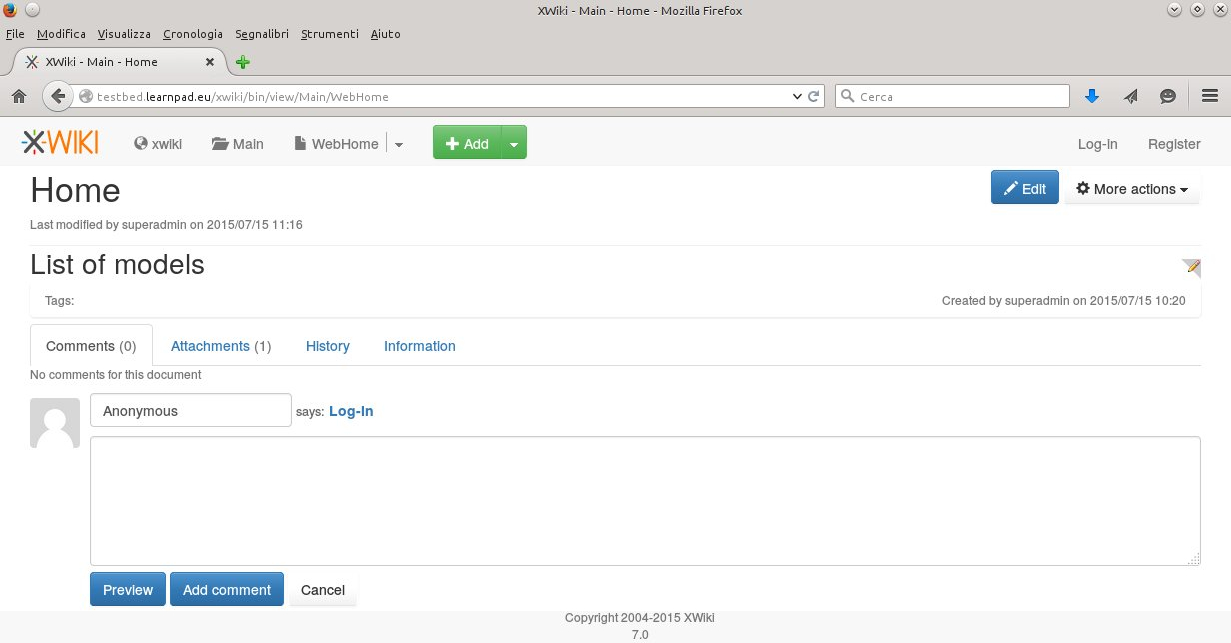
\includegraphics[width=0.85\textwidth]{./Figures/testbed.jpg}
 % testbed.jpg: 1280x1004 pixel, 101dpi, 32.19x25.25 cm, bb=0 0 912 716
 \caption{\learnpad Platform Testbed}
 \label{fig:testbed}
\end{figure}

Note that by accessing the testbed with a browser, it returns the 
web pages of the running instance of the platform. Often, these web pages may 
result or appear empty (see Figure~\ref{fig:testbed}), but this is normal.
In fact, as described above the main purpose of the testbed is to provide
a technical mean to the developers in order to test their components; thus the 
most proper way of interacting with the testbed is not with a browser, yet.
Also, since it's a testing server, data may be erased either at each new
deployment, or periodically.

In this platform, you are able to upload a new model from one of our Modelling
tools (e.g. MagicDraw or ADOxx).  Modelling tools are then able to verify the 
models (please refer to deliverable D4.1~\cite{learnpad:D4.1} for more details 
about the verification process). Once the models has been verified, they are 
imported into the wiki.

All imported models are listed in the main page and you can browse them.  For
each element of the model, a \textit{feedback} button is available at the 
bottom. If the civil servant, looking at the model, want to give a feedback 
about the current page he's browsing, he can through this buttons.  All of 
these feedbacks are aggregate and sent to the modelling tools when asked.  The 
modeller can then try to address the feedbacks in order to improve the models.

% ---------------------------------- Start whit annexes here!
% ----------------------------------

% \annex{}

% ---------------------------------- Start EndNotes here!  
% ---------------------------------- 

% Plese use this command if and only if your text includes endnotes.
% Otherwise, comment it.

% \theendnotes

% ---------------------------------- Bibliography starts here
% ----------------------------------

\bibliographystyle{plain} 
\bibliography{biblio}

\end{document}  
